
\section{Building process}
As seen from Figure \ref{Fig:Build_process}, the building process is composed by various phases:
\begin{itemize}
	\item Using an editor, you create the source and header files.
	\item The makefile defines which operations are needed to complete the build and which files have to be build.
	\item The preprocessor analyzes the source code and runs the preprocessor directives: macros, \#defines, ecc.. are expanded in "normal code": the full source is now ready to be compiled and goes in one *.i file. This operation can be seen by stopping the building process with the command \code{g++ -E main.c -o hello.i}
	\item After compiling the *.i files we get the assembly code, another human-readable text file. This output file can be seen by stopping the building process with the command \code{g++ -c hello.c}
	\item The next step is assembling the code: an *.o (object) file is generated, that's something really close the machine code, but still not hardware dependent: the memory addresses are still relative and the library calls are still not included.
	\item The final step is linking: it adds the static libraries to the code and generates the final executable file.
\end{itemize}
\begin{figure}[h]
	\centering
	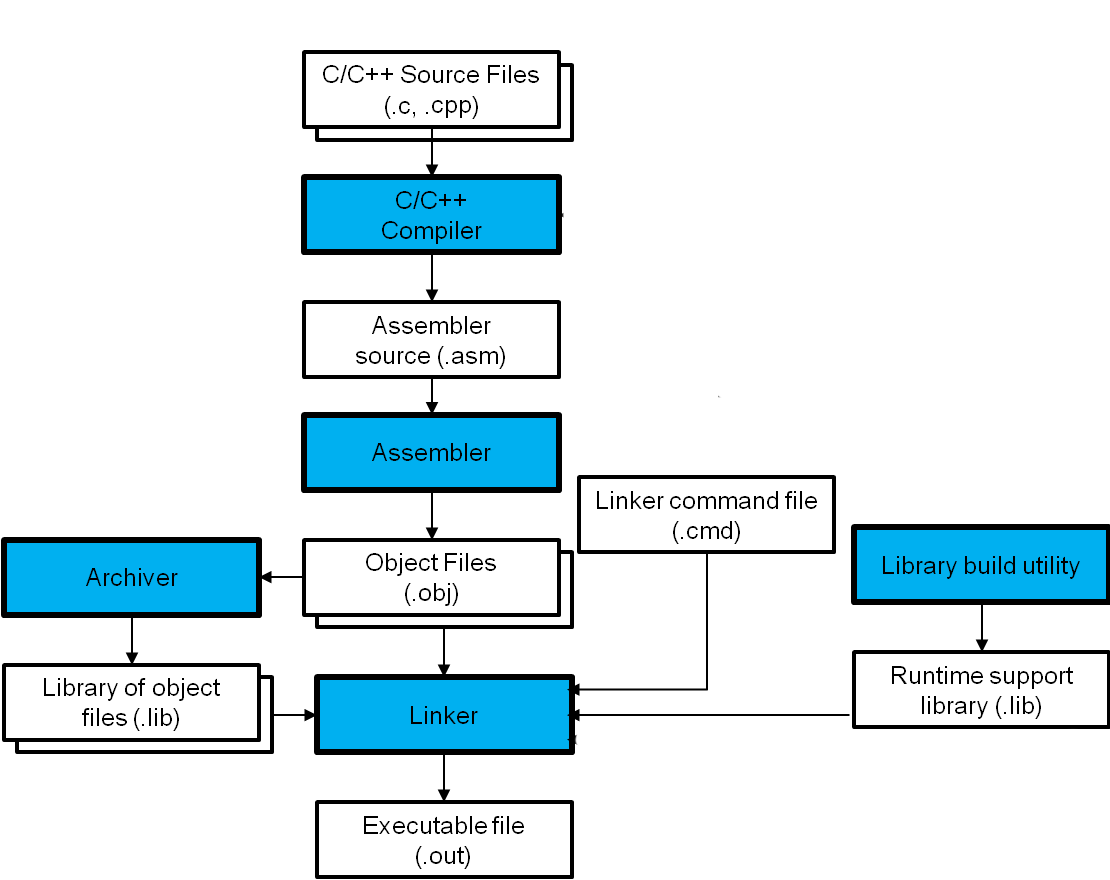
\includegraphics[width=\textwidth]{gfx/build_process}
	
	\caption{Build Process Procedure}
	\label{Fig:Build_process}
\end{figure}

\pagebreak

\section{Makefile}
\subsection{Introduction}
The makefile is a build automator file: when we call the \code{make} command, it tells which files have to be recompiled, relinked, executed, eccc.

Makefiles have 5 types of rules
\begin{itemize}
	\item Explicit goals: they specify how to update a specific file (i.e. main.cpp or main.o)
	\item Implicit goals: they specify how to update a generic class of files (i.e. *.c or *.o)
	\item Variable definition: useful to keep the file reusable in different conditions, by just editing a part of it (if we define the variable \code{NAME=main} in the head of the file, we can use it in the rest of the code )
	\item Directives: they specify when to read other makefiles and when we don't need some parts of the code (where to jump)
	\item Comments: to describe the makefile code, they start with \#%\sharp;
\end{itemize}

\subsection{A goal structure}
A goal is always composed by
\begin{lstlisting}
target : prerequisites
	commands
\end{lstlisting}
in which:
\begin{itemize}
\item Target: are the output files	
\item Prerequisites: are the files on which the \code{Targets} depend
\item Commands: the commands that have to be executed to built the \code{Targets} files starting from the \code{Prerequisites} files.
\end{itemize}

Every file name has to be seen as

\begin{lstlisting}
[p]stem[s].ext
\end{lstlisting}
in which:
\begin{itemize}
	\item \code{p} is the prefix, in common with every file of the class.
	\item \code{stem} is the unique part of the file, that makes it different from the others. In the code is represented by \%.
	\item \code{s} is the suffix, in common with every file of the class.
	\item \code{ext} is the extension, in common with every file of the class.
\end{itemize}
To write implicit goals, we can use:
\begin{itemize}
	\item "\$ @" is the target
	\item "\$ \textless"  is the first prerequisite
	\item "\$ ?" all the recently edited prerequisites
	\item "\$ \textasciicircum" all the prerequisites
	\item "\$ *" the \code{stem} assigned to \%
	
\end{itemize}
\pagebreak
\subsection{Code Example}

\begin{lstlisting}[language=make, basicstyle=\ttfamily \scriptsize]
OUTPUT= main #output file name, changing it here will change it in the whole file
OBJ= main.o #object file(s) name 
CXX=g++	#the name of the compiler, it could be omitted if you call it CXX: its a standard variable
CXXVARS= -Wall -std=c++11 -c #compilation variables: show warnings, compile with c++11 
			     #and stop the compilation at the object creation (do not link the file)

all:$(OUTPUT)  #if i call "make" without parameters i jump here

$(OUTPUT):$(OBJ) #meaning: please generate a $(OUTPUT) file name starting 
		  #from the $(OBJ) object file and, if not present, execute the command
$(CXX) $^ -o $@   #g++ main.o -o main #the command to be executed

%.o:%.cpp	#meaning: please generate a whatever.o object file for every whatever.cpp file. 
		#If the object file is not present, execute the command
$(CXX) $< $(CXXVARS) #the command is g++ whatever.cpp -Wall -std=c++11 -c

clean: #if someone calls "make clean"
rm -f *.o #remove every object file
rm -f $(OUTPUT) #remove every output file

diocane: #if someone calls "make diocane"
./$(OUTPUT) #execute the output file


\end{lstlisting}



\section{Linker Script}
The linker script is a file that defines where the various parts of the compiled code are actually stored in memory.

The simplest possible linker script has just one command:\code[SECTIONS]. This command describes the memory layout of the building output file.

Let's assume that the program consists only of code, initialized data and uninitialized data: these will be, respectively, stored in the \code{.text}, \code{.data} and \code{.bss} sections.

The linker script that could place these section in the correct parts of the memory would be something like:

\begin{lstlisting}
SECTIONS
{
	. = 0X10000; /* everything starts at this address*/
	.text : {*(.text)} /*every text file goes here*/ 
	. = 0x8000000; /*everthing after will be shifted at this */
	.data : { *(.data)}
	.bss : {*.(.bss)}

}

\end{lstlisting}

\subsection{Keywords}
The linker script has the following keywords:
\begin{itemize}
	\item \code{ENTRY(main)}, this is the symbol name for the entry point of the linked program/kernel. It can be "start" or "main" or whatever.It's the first byte of the program (of the first byre of the .txt section in ELF.)
	\item \code{OUTPUT(kernel.bin)}, specifies the file that has to be output by the linker
	\item \code{MEMORY}, declares one or more memory regions with attributes specifuing whether the region can be written to, read from or executed.
	\item \code{ALIGN(4)} instructions tells the linker that this section ought to be word aligned. When you use a 32-bit machine it typically needs to be word aligned (32-bit -> 4 bytes hence the '4' specified with the align command. )
	\item \code{AT} defines the location in FLASH for the RAM data at startup. \\ Can be both used as \code{data: AT(_last_text_address)\{\}} (at data section start) or as \code{\} > ram AT > rom} at the end of the data section.
	\item \code{KEEP(*(.isr_vector))}, is useful to tell the linker to keep (don't erase) those sections that no one calls anywhere in the \code{*.s} file. It's almost the same thing as the \code{volatile} for C. Without this command, some parts may not work at all.
\end{itemize}

Here an example, well documented here:  \url{http://www.hertaville.com/a-sample-linker-script.html}.

\begin{lstlisting}
	/* Entry Point */
	ENTRY(Reset_Handler)
	
	/* Specify the memory areas */
	MEMORY
	{
	FLASH (rx)      : ORIGIN = 0x08000000, LENGTH = 0x10000 /*64K*/
	RAM (xrw)       : ORIGIN = 0x20000000, LENGTH = 0x02000 /*8K*/
	}
	
	/* define stack size and heap size here */
	stack_size = 1024;
	heap_size = 256;
	
	/* define beginning and ending of stack */
	_stack_start = ORIGIN(RAM)+LENGTH(RAM);
	_stack_end = _stack_start - stack_size;
	
	/* Define output sections */
	SECTIONS
	{
	/* The startup code goes first into FLASH */
	.isr_vector :
	{
	. = ALIGN(4);
	KEEP(*(.isr_vector)) /* Startup code */
	. = ALIGN(4);
	} >FLASH
	
	/* The program code and other data goes into FLASH */
	.text :
	{
	. = ALIGN(4);
	*(.text)           /* .text sections (code) */
	*(.text*)          /* .text* sections (code) */
	*(.rodata)         /* .rodata sections (constants, strings, etc.) */
	*(.rodata*)        /* .rodata* sections (constants, strings, etc.) */
	*(.glue_7)         /* glue arm to thumb code */
	*(.glue_7t)        /* glue thumb to arm code */
	. = ALIGN(4);
	_etext = .;        /* define a global symbols at end of code */
	} >FLASH
	
	.ARM.extab   : { *(.ARM.extab* .gnu.linkonce.armextab.*) } >FLASH
	.ARM : {
	__exidx_start = .;
	*(.ARM.exidx*)
	__exidx_end = .;
	} >FLASH
	
	/* used by the startup to initialize data */
	_sidata = .;
	
	/* Initialized data sections goes into RAM, load LMA copy after code */
	.data : AT ( _sidata )
	{
	. = ALIGN(4);
	_sdata = .;        /* create a global symbol at data start */
	*(.data)           /* .data sections */
	*(.data*)          /* .data* sections */
	
	. = ALIGN(4);
	_edata = .;        /* define a global symbol at data end */
	} >RAM
	
	/* Uninitialized data section */
	. = ALIGN(4);
	.bss :
	{
	/*  Used by the startup in order to initialize the .bss secion */
	_sbss = .;         /* define a global symbol at bss start */
	__bss_start__ = _sbss;
	*(.bss)
	*(.bss*)
	*(COMMON)
	
	. = ALIGN(4);
	_ebss = .;         /* define a global symbol at bss end */
	__bss_end__ = _ebss;
	} >RAM
	
	. = ALIGN(4);
	.heap :
	{
	_heap_start = .;
	. = . + heap_size;
	_heap_end = .;
	} > RAM
	
	/* Remove information from the standard libraries */
	/DISCARD/ :
	{
	libc.a ( * )
	libm.a ( * )
	libgcc.a ( * )
	}
	
	.ARM.attributes 0 : { *(.ARM.attributes) }
	}
\end{lstlisting}
%\begin{figure}[h]
%	\centering
%	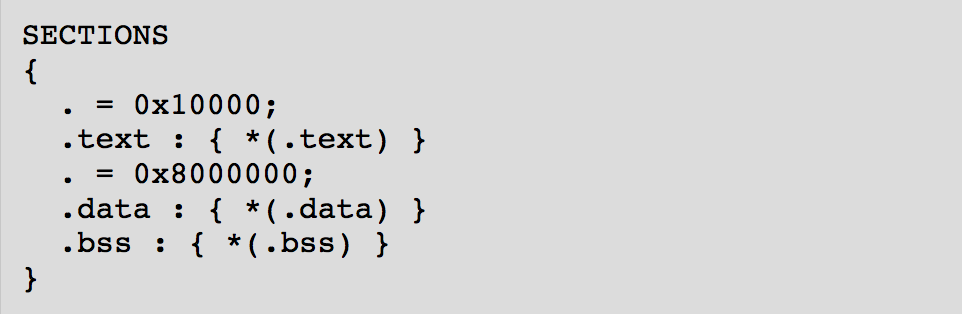
\includegraphics[width=\textwidth/3]{gfx/linker_file}
%	
%	\caption{Linker file example}
%	\label{Fig:Linker File}
%\end{figure}

